\chapter{Introduction}
\section{Dimensional Analysis and SI units}
\subsection{SI Units}
The \index{SI system of units} \gls{siunits} is the standard used by many scientists throughout the world.  There are seven \textit{fundamental} or \textit{base} quantities from which all other measurements are derived.  These quantities are listed below:
 \index{Units, Fundamental}

\begin{center}

	
\begin{table}[ht]\caption{\textbf{SI Units}}% title of Table 
	\centering % used for centering table	
	\begin{tabular}{|c|c|c|}
		\hline \hline
		\textbf{Quantity} & \textbf{Unit} & \textbf{Unit Symbol}\\
		\hline
		time & second & s \\
		\hline
		length & meter & m \\
		\hline
		mass & kilogram & kg \\
		\hline
		electrical current & Ampere & A \\
		\hline
		temperature & Kelvin & K \\
		\hline
		amount of substance & mole & mol \\
		\hline
		luminous intensity & candela & cd \\
		\hline		
	\end{tabular}
	\label{table:nonlin}% is used to refer this table in the text
\end{table}
\end{center}

	Of these quantities, mass, time and length are quite common.  Thus, this system is sometimes called the MKS (meter, kilogram, second) system. In order to use any equations, all measurements must have correct units.  For example, if a time is expressed in hours, it must first be converted into seconds before any calculations can be attempted.  
	
	\subsection{Dimensional Analysis}
	\gls{dimensionalanalysis} \index{Dimensional Analysis} is the process in which the units associated with quantities create \textit{derived units}. \index{Units, Derived} For instance, when a distance is divided by a time, the units will be $ \frac{m}{s}$ (read \textit{meters per second}).  	
	
	Dimensional analysis is an important part of solving physics problems.  Often, correct dimensional analysis can help you determine if a problem has been solved correctly.  One should not even attempt to calculate an answer to a problem until the correct units have been verified. 

	\subsection{Unit Conversions} \index{Unit Conversions}
	Often you will find that you need to convert a measurement from one unit to another.  In order to do this, you must use a \gls{conversionfactor}.  A conversion factor is a fraction that is based upon a statement of equality.  For instance, since 60 seconds = 1 minute, a conversion factor will look like either $\frac{60s}{1 min}$ or $\frac{1 min}{60s}$.  You should chose the version of the conversion factor that eliminates the units that you wish to convert.  
	
	
		\begin{mdframed}[backgroundcolor=blue!10!white]
		\begin{center}
			\textbf{Example \thesubsection}	\label{ex113}
		\end{center}
	
		\vspace{0.1in}	
		\textbf{Problem:} Convert 7.241 hours into seconds. 
		\vspace{0.1in}
		
		\textbf{Solution:} Begin by converting 7.241 hours into minutes.  Since 60 minutes = 1 hour, 
			\begin{equation*}
			7.241 \cancel{hr} \frac{60 min}{1 \cancel{hr}} = 434.46 min
			\end{equation*}
		
		Knowing that 1 minute = 60 seconds, we can use a second conversion factor to obtain seconds:
			\begin{equation*}
			434.46 \cancel{min} \frac{60 s}{1 \cancel{min}} = \boxed{26067.6s}
			\end{equation*}
		
		This problem could be solved in one step if you know that 1 hour = 3600 seconds. 
	
	\end{mdframed}


	
\begin{mdframed}[backgroundcolor=blue!10!white]
	\begin{center}
		\textbf{Example \thesubsection.2}	\label{ex1132}
	\end{center}
	
	\vspace{0.1in}	
	\textbf{Problem:} A car travels with a speed of 20 m/s.  What is this in miles per hour? 
	\vspace{0.1in}
	
	\textbf{Solution:} We begin by converting meters per second into meters per hour:
	\begin{equation*}
	20 \frac{m}{\cancel{s}} \cdot \frac{3600 \cancel{s}}{1 {hr}} = 72000 \frac{m}{hr}
	\end{equation*}
	
	We also need to know that 1 mile = 1609.34 meters:
	\begin{equation*}
		72000 \frac{\cancel{m}}{hr} \cdot \frac{1 mile}{1609.34 \cancel{m}} \approx 44.739 \frac{miles}{hr} 
	\end{equation*}
	
	
\end{mdframed}
		


\section{Vectors and Scalars}
In the study of physics, there are two types of quantities that we will deal with on a regular basis: \textit{scalars} and \textit{vectors}.  

A \gls{scalar} is a quantity that you are already most likely very familiar with, as it is just a number; scalars have only a \gls{magnitude} (a number that represents how big or strong it is), and can sometimes include units.  Examples of scalars might be the number of people in a room, the mass of a car, or your age in years.  

\gls{vector}s are different from scalars because in addition to a magnitude, they contain a direction as well.  Examples of vectors might include 50 feet to the north, 5 m/s at a 33$^\circ$ angle, or 200 miles straight up.  
There are many ways of expressing vectors.  Symbollically, they are often written with an arrow over them.  For example, in the equation \color{blue} $\vec{F} = m \vec{a}$ \color{black}  both force and acceleration are vectors - meaning that both force and acceleration have a direction.  Sometimes vectors will be expressed in \textbf{bold} typeface.   Hence, the expression \\ \color{blue} \textbf{F} = m \textbf{a}  \color{black} is equivalent to the expression shown above.

The direction for vectors in 1 dimension is easy - all you need is a positive or a negative.  Usually, 1-dimensional motion takes place along the x-axis (left and right), but sometimes it will take place in the y- (forward and backward) and z- (up and down) dimensions.  For the purposes of this book, positive is to the right and up unless otherwise stated. 
In two dimensions, a vector requires two pieces of information.  One way of expressing a vector is in polar form.  Polar form in two dimensions includes a magnitude of the vector and an angle, usually measured from the x-axis.  There are several ways for writing this.  4 cm @ 15$^\circ$, \\ 4 cm $\angle 15^\circ$ and 4 cm at 15$^\circ$ North of East all represent the following displacement vector:



\begin{figure}[h]
	\caption{A vector represented graphically.} \label{figure:M1}
	\centering
	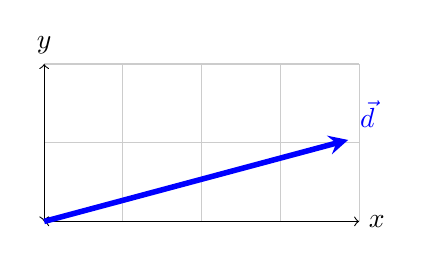
\begin{tikzpicture}
	
	\draw[thin,gray!40] (0,0) grid (4,2);
	\draw[<->] (0,0)--(4,0) node[right]{$x$};
	\draw[<->] (0,0)--(0,2) node[above]{$y$};
	\draw[line width=2pt,blue,-stealth](0,0)--(3.86,1.035) node[anchor=south west]{$\vec{d}$};
	
	
	
	
	\end{tikzpicture}
	
\end{figure}


	
	
	



	
	The magnitude of the above vector is 4 cm.  Mathematically, the magnitude of a vector can be written several ways, the most common being $\lvert \vec{A} \rvert$, though sometimes the magnitude of a vector can be written as the vector without the vector sign, as in $A$. 
	
	\subsection{Unit Vectors}
	\index{Unit Vectors}
	\gls{unitvector} are vectors that have a length of one unit and are oriented along one axis.  The unit vector for the x-direction is written as $\hat{i}$ (pronounced i-hat).  $\hat{i}$ is a 1-unit long vector that is always parallel to the x-axis, and points in the direction of increasing x values.  Likewise, the y-direction and z-direction unit vectors are written as $\hat{j}$ and $\hat{k}$ respectively.  
	
	
	Because the surface of a paper is effectively 2-dimensional, it is very hard to draw lines that are oriented directly into or out of your paper. For this purpose, physicists have agreed to the following convention: vectors that point directly into your paper are notated by $\bigotimes$ .  Vectors that point directly out of your paper are shown by the symbol $\bigodot$.  
	
	Sometimes, vectors may be expressed in Cartesian coordinates.  This vector could either be expressed as an ordered pair (or triple) with square brackets, such as [3, 4, 5] cm, or as a linear combination of the unit vectors shown above, such as $5\hat{i} + 12 \hat{j} + 3 \hat{k}$  In each case, the distances in each direction are given by the numbers shown.  The vector in figure \ref{figure:M1} could be represented as: \color{blue} $\vec{d}  \approx 3.86 \hat{i} + 1.035 \hat{j}$.  \color{black}
	
	When converting between polar and cartesian forms for two dimensional vectors, a little trigonometry shows: 
		\begin{mdframed}[backgroundcolor=orange!20!white]
	
	\color{blue}
	\begin{multicols}{2}
		\begin{center}
			\begin{equation}
			x = r \cos(\theta)
			\label{eq11}
			\end{equation}
			
			\begin{equation}
			y = r \sin(\theta)
			\end{equation}

			\begin{equation}
			r = \sqrt{x^2+y^2}			
			\end{equation}

			\begin{equation}
			\theta=\tan^{-1}(\frac{y}{x})
			\label{eq14}
			\end{equation}		
		\end{center}
	\end{multicols}
	\color{black}
	\end{mdframed}
	
	In three dimensions, polar form comes in two types: \textbf{cylindrical} and \textbf{spherical}.  In cylindrical coordinates, expressed as [r, $\theta$, z],  the above conversions are used, and the z-coordinate remains unchanged from Cartesian form.  In spherical coordinates, the vector [r, $\theta$, $\phi$] includes a radial distance, an azimuthal angle and a polar angle. 

	
	
	
	
\section{Vector Mathematics}
	\subsection{Vector Addition} \index{Vectors, Addition}
	\subsubsection{Graphical Addition of Vectors} 
	When vectors are added graphically, they are added \textbf{head} to \textbf{tail}.  This means that the arrowhead for a first vector becomes the origin for the second vector.  The \gls{resultant} vector is a straight line between the origin of the first vector and the head of the second.  
	
	
	\begin{mdframed}[backgroundcolor=blue!10!white]
		\begin{center}
			
			
			\textbf{Example \thesubsection}	\label{test}
		\end{center}
		
		\vspace{0.1in}
		\textbf{Problem:}  If $\vec{A} =  \hat{i} + 2 \hat{j} $ and $\vec{B} = 3 \hat{i} - \hat{j} $, 
		find $\vec{C}$ graphically given $\vec{C} = \vec{A} + \vec{B}$ 
		
		\vspace{0.1in}
		
		
		\textbf{Solution:} Begin by drawing $\vec{A}$:
		
		
			
		
		\begin{center}
			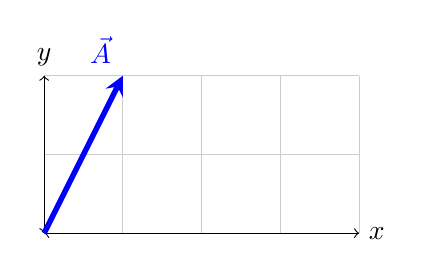
\begin{tikzpicture}
			\draw[thin,gray!40] (0,0) grid (4,2);
			\draw[<->] (0,0)--(4,0) node[right]{$x$};
			\draw[<->] (0,0)--(0,2) node[above]{$y$};
			\draw[line width=2pt,blue,-stealth](0,0)--(1,2) node[anchor=south east]{$\vec{A}$};

			\end{tikzpicture}
			
		\end{center}
	
		Now use the head of $\vec{A} $ as the origin for $\vec{B}$:
	
	
		\begin{center}
		
		
		
		
		
		
		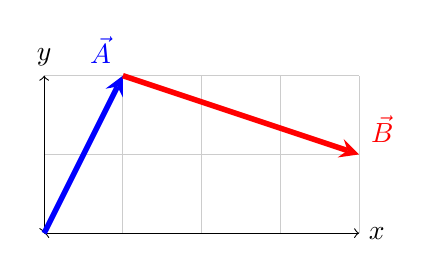
\begin{tikzpicture}
		\draw[thin,gray!40] (0,0) grid (4,2);
		\draw[<->] (0,0)--(4,0) node[right]{$x$};
		\draw[<->] (0,0)--(0,2) node[above]{$y$};
		\draw[line width=2pt,blue,-stealth](0,0)--(1,2) node[anchor=south east]{$\vec{A}$};
		\draw[line width=2pt,red,-stealth](1,2)--(4,1) node[anchor=south west]{$\vec{B}$};

		\end{tikzpicture}		
		
	\end{center}
	
	The resulting vector is a straight line from the origin to the end of $\vec{B}$: 
	
	
	\begin{center}
		

		
		
		
		
			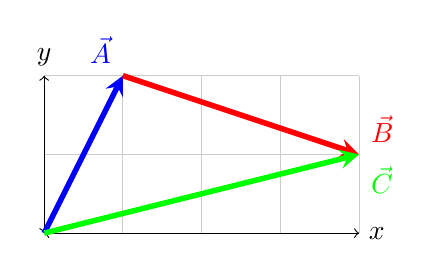
\begin{tikzpicture}
			\draw[thin,gray!40] (0,0) grid (4,2);
			\draw[<->] (0,0)--(4,0) node[right]{$x$};
			\draw[<->] (0,0)--(0,2) node[above]{$y$};
			\draw[line width=2pt,blue,-stealth](0,0)--(1,2) node[anchor=south east]{$\vec{A}$};
			\draw[line width=2pt,red,-stealth](1,2)--(4,1) node[anchor=south west]{$\vec{B}$};
			\draw[line width=2pt,green,-stealth](0,0)--(4,1) node[anchor=north west]{$\vec{C}$};
			\end{tikzpicture}
			
			
			
		\end{center}
		
		The resultant vector is given by $\boxed {\vec{C} = 4 \hat{i} + \hat{j}}$
		
	\end{mdframed}
	
	\subsubsection{Mathematical Addition of Vectors}
	Mathematical addition of vectors in Cartesian form is quite easy - simply add corresponding x- and y- values together.  For instance, in Example \ref{test} we are given  $\vec{A} =  \hat{i} + 2 \hat{j} $ and $\vec{B} = 3 \hat{i} - \hat{j} $.  Adding these together would give $\vec{C} = (1 +3) \hat{i} + (2-1)\hat{j} \longrightarrow \vec{C} =  4 \hat{i} + \hat{j} $.
	
	The easiest way to add vectors that are expressed in polar coordinates is to first convert them into cartesian coordinates using Equations \eqref{eq11} through \eqref{eq14} on page \pageref{eq11}.
	
	
	
	\subsection{The Dot Product} \index{Dot Product} \index{Vectors, Dot Product}
	\subsubsection{In Cartesian Form}
	When multiplying vectors, it is sometimes necessary to obtain a scalar result.  This is done through use of a \gls{dotproduct}.  A dot product is written as $\vec{A} \cdot \vec{B} $.  This means to only multiply the components of the vectors that are in the same direction.  In cartesian coordinates, this can be done by multiplying corresponding components, then adding the products.  
	
		\begin{mdframed}[backgroundcolor=blue!10!white]
			\begin{center}
				\textbf{Example \thesubsection}	\label{example:dotproduct}
				
				
			\end{center}
		
		\textbf{Problem:} Given the vectors $ \vec{Y} = 2 \hat{i} + 3 \hat{j} $ and $\vec{Z} = -4 \hat{i} + 5 \hat{j}$ find the dot product of vectors Y and Z. 
		
		\vspace{.1in}
		
		\textbf{Solution:} Multiply coefficients from each vector, then add the products together:
		\begin{center}
			$2\times(-4) + 3\times 5 = -8 + 15 = \boxed{7}$ 
		\end{center}
		
		
		\end{mdframed}
	\subsubsection{In Polar Form}
	Often, vectors will be expressed in polar notation.  If this is the case, the dot product can be found my multiplying the magnitude of the first vector times the magnitude of the second vector times the cosine of the angle between:
	
	
	\begin{mdframed}[backgroundcolor=orange!20!white]
		\begin{equation}
			\label{equation:dotproduct}
		\vec{A} \cdot \vec{B} = \lvert \vec{A} \rvert  \lvert \vec{B} \rvert \cos{\theta}
		\end{equation}
		
	\end{mdframed}
	
	
	\vspace{0.1in}
	
	
		\begin{mdframed}[backgroundcolor=blue!10!white]
		\begin{center}
			\textbf{Example \thesubsection.2}	\label{example:dotproduct2}
			\vspace{0.1in}
			
			
		\end{center}
		
		\textbf{Problem:} Given the vectors $ \vec{D} = 3 \angle 30^{\circ} $ and $\vec{E} = 5 \angle 60^{\circ}$ find the dot product of vectors D and E. 
		
		\vspace{.1in}
		
		\textbf{Solution:}  We begin by graphing both vectors starting from a common origin:
		\begin{center}
		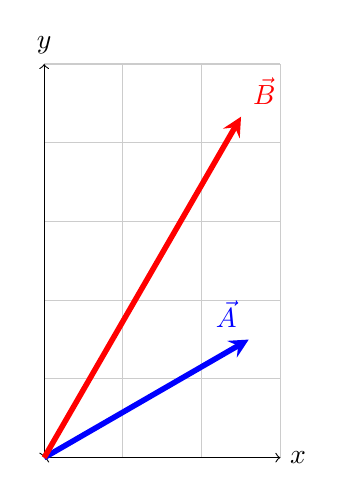
\begin{tikzpicture}
		\draw[thin,gray!40] (0,0) grid (3,5);
		\draw[<->] (0,0)--(3,0) node[right]{$x$};
		\draw[<->] (0,0)--(0,5) node[above]{$y$};
		\draw[line width=2pt,blue,-stealth](0,0)--(2.598,1.5) node[anchor=south east]{$\vec{A}$};
		\draw[line width=2pt,red,-stealth](0,0)--(2.5,4.33) node[anchor=south west]{$\vec{B}$};
		
		\end{tikzpicture}	
			

		\end{center}
			
			Noticing that the angle between the two vectors is $30^\circ$, we can use equation 1.5 to calculate:
			
			\begin{center}
				$ 		\vec{D} \cdot \vec{E} = \lvert \vec{D} \rvert  \lvert \vec{E} \rvert \cos{\theta} = (3)(5)\cos30^\circ \approx \boxed{12.990} $
			\end{center}
		
		
		
		
		\begin{center}
			
		\end{center}
		
		
	\end{mdframed}
	
	
	
	\subsection{The Cross Product}  \index{Cross Product} \index{Vectors, Cross Product}
	\subsubsection{Cross Products In Cartesian Form}
	Sometimes two vectors will be multiplied in such a way that they will result in another vector.  This is called a \gls{crossproduct}.  A cross product is inherently a three-dimensional operation.  A cross product can be found by calculating the \gls{determinant} of a matrix:  
	
\begin{mdframed}[backgroundcolor=orange!20!white]
\begin{equation}
 \vec{A} \times \vec{B} = 	\begin{vmatrix}
				\hat{i} & \hat{j} & \hat{k}\\
				A_x & A_y & A_z \\
				B_x & B_y & B_z 
				\end{vmatrix} 
				\label{equation:16}
\end{equation}
\end{mdframed}	

	
The most common way to find the determinant of the above matrix is by using minors:
\begin{center}
$
 \vec{A} \times \vec{B} = 	\begin{vmatrix}
	\hat{i} & \hat{j} & \hat{k}\\
	A_x & A_y & A_z \\
	B_x & B_y & B_z 
\end{vmatrix} 
= \hat{i} \begin{vmatrix}
	A_y & A_z \\
	B_y & B_z 
\end{vmatrix} - \hat{j} \begin{vmatrix}
A_x & A_z \\
B_x & B_z 
\end{vmatrix} + \hat{k} \begin{vmatrix}
A_x & A_y \\
B_x & B_y 
\end{vmatrix}
$
\end{center}

This finding the determinate of each of the 2x2 matrices yields:
\begin{center}
	$ \vec{A} \times \vec{B} = 	\hat{i} (A_y B_z - A_z B_y) - \hat{j}(A_x B_z - A_z B_x)+ \hat{k}(A_x B_y - A_y B_x)
$\end{center}



	\begin{mdframed}[backgroundcolor=blue!10!white]
	\begin{center}
		\textbf{Example \thesubsection}	\label{example:crossproductcartesian}
		\vspace{0.1in}
		
		
	\end{center}
	
	\textbf{Problem:} Given the vectors $ \vec{V} = 2 \hat{i} + 3 \hat{j} $ and $\vec{W} = -4 \hat{i} + 5 \hat{j}$ find the cross product of vectors V and W. 
	
	\vspace{.1in}
	
	\textbf{Solution:}  Begin by creating a matrix, as shown in equation \eqref{equation:16}.  Since both vectors lie in the X-Y plane, the Z-components for both vectors are zero:
	
	\begin{center}
		$\vec{V} \times \vec{W} =  \begin{vmatrix}
		\hat{i} & \hat{j} & \hat{k} \\
		2 & 3 & 0\\
		-4 & 5 & 0		
		\end{vmatrix}$

	\end{center}

Now, use expansion by minors to create three two-by-two matrices:

\begin{center}
	$\vec{V} \times \vec{W} =  \begin{vmatrix}
	\hat{i} & \hat{j} & \hat{k} \\
	2 & 3 & 0\\
	-4 & 5 & 0		
	\end{vmatrix} = \hat{i} \begin{vmatrix}
		3 & 0 \\
		5 & 0 
	\end{vmatrix} - \hat{j} \begin{vmatrix}
		2 & 0 \\
		-4 & 0 
	\end{vmatrix} + \hat{k} \begin{vmatrix}
		2 & 3 \\
		-4 & 5 
	\end{vmatrix}
	$
\end{center}

Finding the determinate of each of the two-by-two matricies yields: 
\begin{center}
	$	\vec{V} \times \vec{W} = \hat{i}(3\cdot0-0\cdot5)-\hat{j}(2\cdot0-0\cdot(-4))+\hat{k}(2\cdot5-3\cdot(-4))$
\end{center}

Both the x-component and the y-components of this cross product are zero.  Thus, 
\begin{center}
	$	\boxed{\vec{V} \times \vec{W} = 22 \hat{k}}$
\end{center}


\end{mdframed}
	
	There are some important things you may wish to note.  
	\begin{enumerate}
		\item The cross product is not commutative.  That is, $\vec{A} \times \vec{B} \neq \vec{B} \times \vec{A}$.  In fact, the two cross products are in exactly opposite directions.  
		\item The cross product of two vectors is always a vector that is perpendicular to both of the original vectors.  
	\end{enumerate}


\subsubsection{Cross Products In Polar Form}
	When vectors are expressed in polar form, a cross product can often be found using two steps.  To find the magnitude of the resulting vector, one would use the following equation:
	
\begin{mdframed}[backgroundcolor=orange!20!white]
	\begin{equation}
	\lvert \vec{A} \times \vec{B} \rvert = 	\lvert \vec{A} \rvert \lvert\vec{B} \rvert \sin \theta
	\label{Equation:17}
	\end{equation}
\end{mdframed}	

\label{RHR1}
In Equation \ref{Equation:17}, $\theta$ is the angle between the two vectors.  To find the direction of the resulting vector, use the \gls{righthandrulefirst}.  \index{Right Hand Rule, First} \index{First Right Hand Rule} To use this rule, you point your index finger in the direction of the first vector to be multiplied.  Your middle finger is then pointed in the direction of the second vector to be multiplied.  Your thumb will point in the direction of the resultant vector, as shown in the image: 

\begin{center}
	\begin{figure}[h]
		\centering
	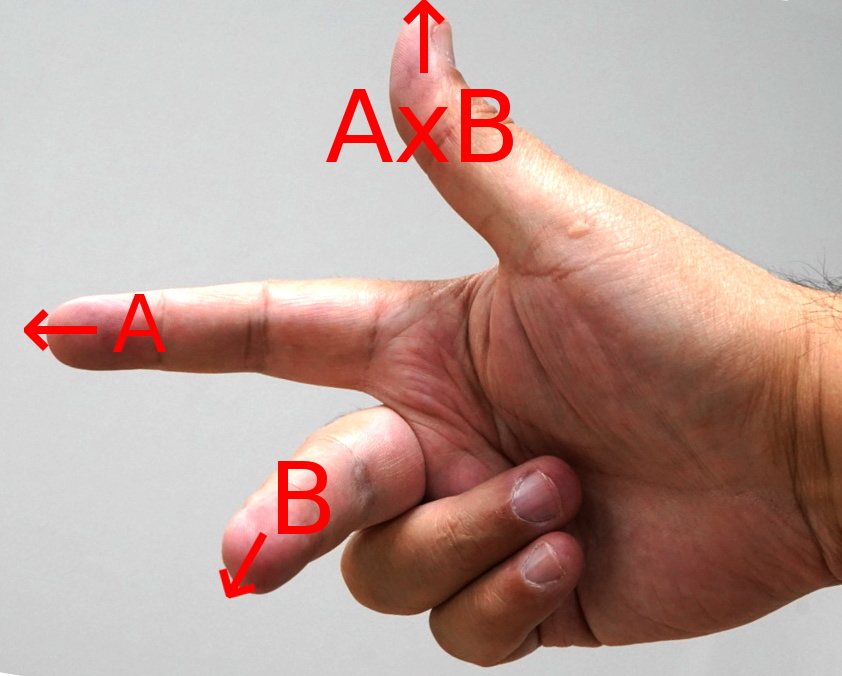
\includegraphics[height=2in]{./Chapters/Ch01-intro/righthandrule.JPG}	
	\caption{The First Right Hand Rule}
	\end{figure}
	
\end{center}

The right had rule is easiest to use when the first two vectors are at $90^\circ$ to each other.  However, even if the first two vectors are not at right angles to each other, the resultant vector of a cross product will always be perpendicular to the plane of the first two vectors.  


%\newpage
%\section{Exercises for Chapter 1}

%\begin{multicols}{2}


%	\begin{enumerate}


%	\subsection*{Section 1.1: Dimensional Analysis}
%		\item What are the units for each of the following?
%			\begin{enumerate}
%				\item $\frac{5 m}{2 s}$
%				\item $\frac{10kg}{5s}$
%				\item $\frac{140 kg \cdot 15 m}{23 s} $
%				\item $\frac{(\frac{15m}{15s})}{14 s} $
%				
%			\end{enumerate}
%	\subsection*{Section 1.2: Vectors and Scalars}
%		\item Given the vector $4\hat{i} - 3 \hat{j}$, represent the vector (a) graphically and (b) in polar form.  
%		\item George walks 200 meters north, then walks 400 meters north.  What is the vector from his starting position to his %nding position in (a) cartesian form and (b) polar form (take north as 0 degrees).  
%	\subsection*{Section 1.3: Vector Mathematics}
%		\item Addition - cartesian
%		\item Addition - polar
%		\item Dot Product - Cartesian
%		\item Dot Product - polar
%		\item Cross Product - cartesian
%		\item Cross Product - polar
%		
%		
%	\end{enumerate}	
%\end{multicols}	
	



